\chapter{LPWAN}
\label{chapter:lpwan}

LPWAN (Low-Power Wide-Area Network) je tehnologija za bežičnu komunikaciju na širokom području uz nisku potrošnju električne energije. Zbog zahtjeva za komunikacijom u M2M (Machine to Machine) i IoT (Internet of Things) sustavima razvijaju se mnoge LPWAN tehnologije te su dokaz današnjeg trenda evolucije telekomunikacija. Fokus ovog rada je jedna od tih tehnologija.
\newline

\section{Karakteristike}
\label{section:lpwan_karakteristike}
Komunikacija niske potrošnje energije uz nižu cijenu tehnologije u odnosu na slučaj sa tradicinonalnim mobilnim mrežama jedan je od aduta LPWAN tehnologija. Također i podrška za veći broj spojenih uređaja na većem geografskom području.
\newline
Tipične veličine paketa u LPWAN-u su između 10B i 1kB uz brzine prijenosa do 200kbps. Najčešća topologija u ovakvim mrežama je zvijezdasta gdje se krajnje točke spajaju na zajedničku pristupnu točku kao i kod WiFi tehnologije.
\newline

Neke od najpoznatijih LPWAN tehnologija su: \begin{itemize}
\item Sigfox
\item Lora
\item NB-IoT (Narrowband-IoT)
\item LTE-M
\item Nwave
\item RPMA
\end{itemize}

\begin{figure}[ht!]
\centering
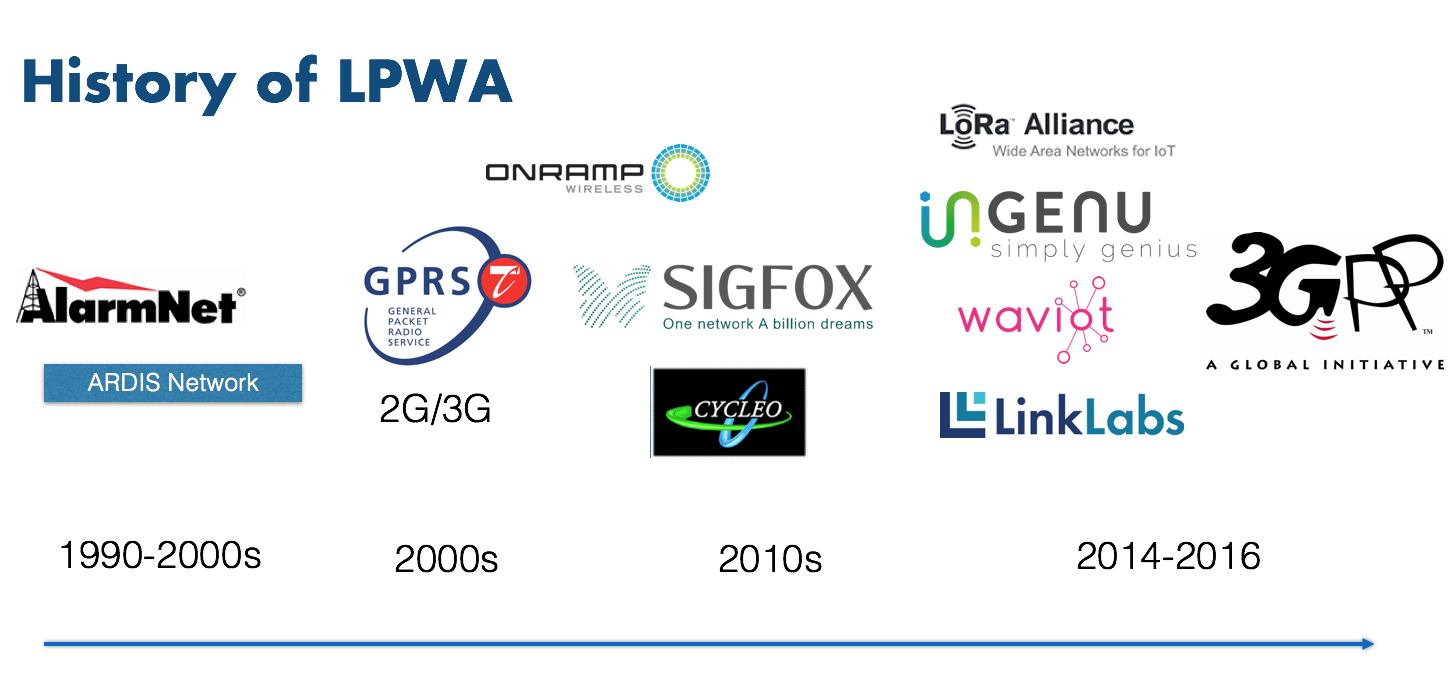
\includegraphics[width=1.0\textwidth]{images/lpwan_history.png}
\caption{Pregled LPWAN tehnologija kroz povijest}
\label{img:lpwan_overview}
\end{figure}

\pagebreak
S obzirom na velik broj raspoloživih tehnologija gdje svaka nudi nešto drugačije teško je ili nemoguće reći koja je najbolja. Možemo predpostaviti da će potrebe IoT-a i ostalih primjena dalje pogoniti razvoj te da će se kroz par godina iskristalizirati situacija među morem raspoloživih tehnologija.
Pri odabiru tehnologije za konkretnu primjenu odnosno projekt potrebno je svakako sagledati sve prednosti i mane pojedine tehnologije.
\newline

Najbitnije karakteristike LPWAN mreža:
\begin{itemize}
\item Mala potrošnja električe energije - omogućuje dugotrajan rad baterijski napajanih uređaja (do 10 ili više godina)
\item Komunikacija na velike udaljenosti
\item Moguć velik broj sudionika u mreži (visok kapacitet mreže)
\item Potrebno malo baznih stanica (u odnosu na mobilne mreže)
\item Korištenje uglavnom nelicenciranog spektra (LoRa i Sigfox)
\item Niska cijena komunikacijskih modula/chipseta (mala kompleksnost sklopovlja)
\item Niska latencija
\end{itemize}

\vspace{5mm}
Najčešći zahtjevi M2M i IoT sustava, a koji nisu dobro podržani tradicionalnim tehnologijama su potreba za komunikacijom na velike udaljenosti i na velikom području te najčešće prijenos male količine podataka te vrlo mala frekvencija slanja ili primanja podataka (čak do samo par poruka dnevno).
Ovi zahtjevi uzeti su u obzir pri dizajniranju LPWAN tehnologija. Kako bi navedeni zahtjevi mogli biti zadovoljeni napravljen je kompromis na štetu brzine prijenosa podataka, što za M2M i IoT primjene najčešće nije problem zbog male količine podataka koju je potrebno prenjeti.
Usporedba LPWAN mreže s ostalim mrežama prikazana ja na slici \ref{img:comparison}.
\begin{figure}[ht!]
\centering
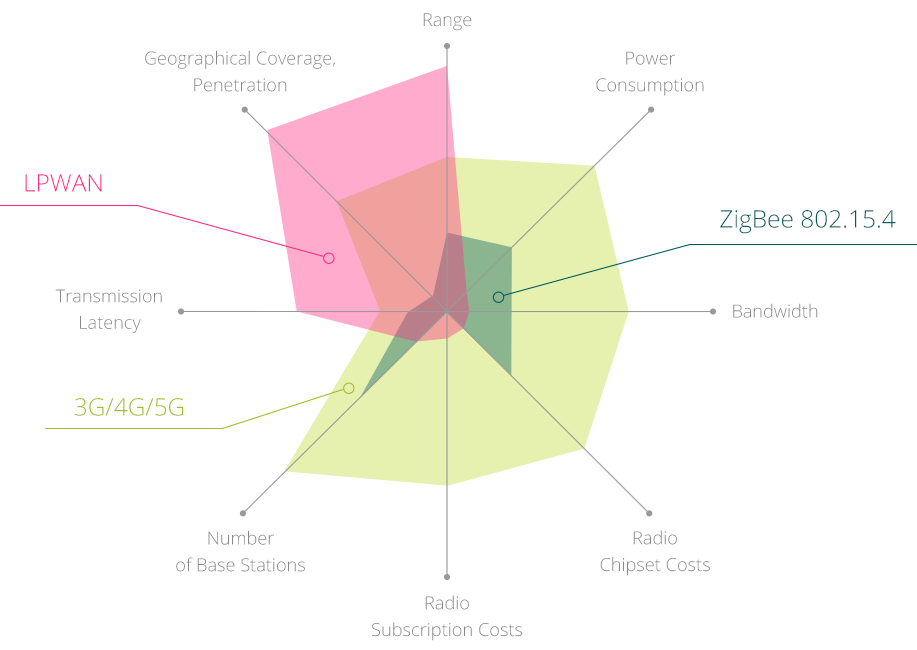
\includegraphics[width=1.0\textwidth]{images/lpwan_other_comparison.png}
\caption{Usporedba bežičnih komunikacijskih mreža}
\label{img:comparison}
\end{figure}

\section{Primjena}
\label{section:lpwan_primjena}
Moguća područja za primjenu neke od LPWAN tehnologija su sva gdje je potreban prijenos male količine podataka na velike udaljenosti uz minimalnu potrošnju električne energije odnosno minimalnu potrošnju baterije ako su krajnji uređaji napajani baterijski.

\pagebreak
Područja primjene i neki aktualni primjeri:
\begin{itemize}
\item Pametni gradovi (pametni semafori, pametna rasvjeta i sl.)
\item Transport
\item Precizna poljoprivreda (npr. određivanje idealnog trenutak za sjetvu ili praćenje parametara tla)
\item Senzorske mreže
\item Telemedicina
\item Praćenje parametara iz prirode (npr. predviđanje potresa i zagađenja zraka)
\item Praćenje parametara infrastrukture (npr. mostovi i tuneli)
\end{itemize}


\begin{figure}[ht!]
\centering

\includegraphics[width=0.8\textwidth]{images/use_cases.png}
\caption{Područja primjene LPWAN tehnologija}
\label{img:comparison}
\end{figure}

